\documentclass[aspectratio=169,11pt,usenames,dvipsnames,handout]{beamer}

\usepackage[english]{babel}
\usepackage{graphicx}
\usepackage{enumitem}
\usepackage{amsmath}
\newlength{\dhatheight}
\newcommand{\doublehat}[1]{%
    \settoheight{\dhatheight}{\ensuremath{\hat{#1}}}%
    \addtolength{\dhatheight}{-0.2ex}%
    \hat{\vphantom{\rule{1pt}{\dhatheight}}%
    \smash{\hat{#1}}}}
\usepackage{mathtools}
\usepackage{float}
\usepackage{tikz}
\usetikzlibrary{patterns,arrows.meta,calc,3d,angles}
\usepackage{tkz-euclide}
\tikzset{point style/.style = {%
  draw = black,
  inner sep = 0pt,
  shape = circle,
  minimum size = 5pt,
  fill = black
 }
}
\usepackage{enumitem}

\usepackage{caption}
\usepackage{subcaption}

\usepackage{booktabs}
% Flowchart stuff

\usepackage{pgfopts}
\usepackage{xcolor}
\usepackage{tcolorbox}

\usetheme[
 titlestyle=style2,
 titleformat=smallcaps,
 sectionstyle=plain,
 slidestyle=cyber,
 headingcolor=theme,
 block=transparent
]{trigon}

\title{Number Sets}
\date{\today}
\author{Adam Klepáč}
\institute[GEVO]{Gymnázium Evolution Jižní Město}
\biglogo[width=.2\textwidth]{logo}
\smalllogo[width=.1\textwidth]{logo}
\titlegraphic{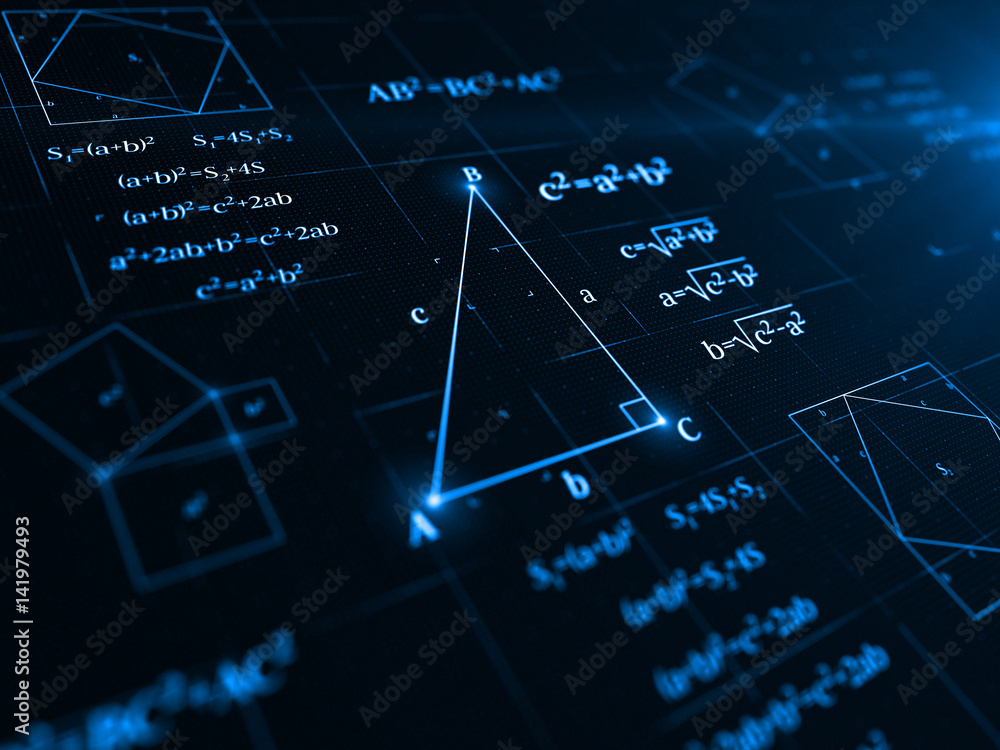
\includegraphics[height=\paperheight]{title.jpg}}

\def\subsectionname{}

% enumerate and itemize global settings
\setlist{topsep=0pt}
\setlist[itemize,1]{label=\textbullet}
\setlist[enumerate,1]{label=\arabic*.}
\setlist[enumerate,2]{label=\alph*)}

% custom colors %
\definecolor{Tiber}{HTML}{0A2841}
\definecolor{Charlotte}{HTML}{C0F6F9}
\definecolor{PictonBlue}{HTML}{53D0EC}
\definecolor{CuriousBlue}{HTML}{228FC6}
\colorlet{tPrim}{PictonBlue}
\colorlet{tTheme}{Charlotte}
\colorlet{tSec}{Tiber}
\colorlet{tAccent}{Tiber}

\newcommand{\clt}{\textcolor{Tiber}}
\newcommand{\clc}{\textcolor{Charlotte}}
\newcommand{\clp}{\textcolor{PictonBlue}}
\newcommand{\clu}{\textcolor{CuriousBlue}}
\newcommand{\clr}{\textcolor{BrickRed}}
\newcommand{\clb}{\textcolor{RoyalBlue}}
\newcommand{\clg}{\textcolor{ForestGreen}}
\newcommand{\clm}{\textcolor{Magenta}}
<<<<<<< HEAD
\newcommand{\cls}{\textcolor{Salmon}}
=======
>>>>>>> 234d6d09a06d1f32ff20f07bf17e192dc1f51a20

\newcommand{\N}{\mathbb{N}}
\newcommand{\Z}{\mathbb{Z}}
\DeclareMathOperator{\tng}{\triangle}

\tcbset{
 boxsep=7pt,
 fonttitle=\sc,
 colframe=tGreyBg,
 colframe=CuriousBlue,
 boxrule=1pt
}

\begin{document}
\titleframe

\begin{frame}
 \frametitle{Contents}
 \tableofcontents
\end{frame}

\section{Natural Numbers}

\begin{frame}
 \frametitle{Natural Numbers -- Intuition}
 \alert{Natural numbers} are intuitively objects which represent a
 \alert{quantity}.\\
 \pause
 They're the following set:
 \[
  \N = \{0,1,2,3,\ldots\}.
 \]
 \pause
 A good way to think about them is to view them as `\emph{collections of
 blocks}'. You get the next natural number by adding another block on top of the
 previous collection.
 \begin{center}
  \begin{tikzpicture}
   \node at (0,-0.3) {$0$};

   \node at (1,-0.3) {$1$};
   \draw[draw=Tiber,thick,fill=PictonBlue] (0.85,0) rectangle ++(.3,.3);

   \node at (2,-0.3) {$2$};
   \draw[draw=Tiber,thick,fill=PictonBlue] (1.85,0) rectangle ++(.3,.3);
   \draw[draw=Tiber,thick,fill=PictonBlue] (1.85,0.4) rectangle ++(.3,.3);

   \node at (3,-0.3) {$3$};
   \draw[draw=Tiber,thick,fill=PictonBlue] (2.85,0) rectangle ++(.3,.3);
   \draw[draw=Tiber,thick,fill=PictonBlue] (2.85,0.4) rectangle ++(.3,.3);
   \draw[draw=Tiber,thick,fill=PictonBlue] (2.85,0.8) rectangle ++(.3,.3);

   \node at (4,-0.3) {$\ldots$};
  \end{tikzpicture}
 \end{center}
\end{frame}

\begin{frame}
 \frametitle{Natural Numbers -- Def\hspace*{0pt}inition}
 There are many ways to define natural numbers.\\
 \pause
 One of the popular ones is using a \alert{successor} function, denoted $s$.
 \pause
 If $n$ is a natural number, then $s(n)$ basically means `add another block on
 top of $n$'.\\
 \pause
 One would be of course tempted to write
 \[
  s(n) = n + 1
 \]
 but that \alert{doesn't make any sense}. We \alert{don't have addition yet}! In
 fact, you need the successor function to define addition in the first place.
\end{frame}

\begin{frame}
 \frametitle{Natural Numbers -- Def\hspace*{0pt}inition}
 The following \alert{five axioms} (often called \emph{Peano axioms}) constitute
 the definition of natural numbers:
 \pause
 \begin{enumerate}
  \item There exists the natural number $0$.
  \pause
  \item Every natural number has a successor which is also natural.
  \pause
  \item The number $0$ is not the successor of any natural number.
  \pause
  \item If $s(n) = s(m)$, then $n = m$.
  \pause
  \item (Induction Axiom) If a statement is true for $0$ and it being true for
   $n$ also implies that it is true for $s(n)$, then it is true for all natural
   numbers.
 \end{enumerate}
\end{frame}

\subsection{Unpacking The Axioms}

\begin{frame}
 \subsectionpage
\end{frame}

\begin{frame}
 \frametitle{Natural Numbers -- Axiom 1}
 \begin{center}
  \Large There exists the natural number $0$.\\
  \pause
  \vspace{\parskip}
  \normalsize\textcolor{Gray}{Hopefully obvious.}
 \end{center}
\end{frame}

\begin{frame}
 \frametitle{Natural Numbers -- Axiom 2}
 \begin{center}
  \Large Every natural number has a successor which is also natural.\\
  \pause
  \vspace{\parskip}
  \normalsize\textcolor{Gray}{Basically means that the natural numbers are an
  infinite set. You can add another block atop any collection of blocks.}
 \end{center}
\end{frame}

\begin{frame}
 \frametitle{Natural Numbers -- Axiom 3}
 \begin{center}
  \Large The number $0$ is not the successor of any natural number.\\
  \pause
  \vspace{\parskip}
  \normalsize\textcolor{Gray}{Basically means that the natural numbers are
  infinite only `in one direction'. There is a \textbf{first} natural number.}
 \end{center}
\end{frame}

\begin{frame}
 \frametitle{Natural Numbers -- Axiom 4}
 \begin{center}
  \Large If $s(n) = s(m)$, then $n = m$.\\
  \pause
  \vspace{\parskip}
  \normalsize\textcolor{Gray}{This means that the successor function is
  \textbf{injective} -- each natural number has a different successor.}
 \end{center}
\end{frame}

\begin{frame}
 \frametitle{Natural Numbers -- Axiom 5}
 \begin{center}
  \Large If a statement is true for $0$ and it being true for $n$ also implies
  that it is true for $s(n)$, then it is true for all natural numbers.\\
  \pause
  \vspace{\parskip}
  \normalsize\textcolor{Gray}{This means that any feature of the natural
   numbers `propagates' via the successor function. Basically, if something is
   true for $0$ and we know that it is true for the next natural number if it is
   true for the previous one, then it is true for $1$ as well. Because it true
   for $1$, it is true for $2$ as well, etc.}
 \end{center}
\end{frame}

\subsection{Operations On Natural Numbers}

\begin{frame}
 \subsectionpage
\end{frame}

\begin{frame}
 \frametitle{What Is An Operation?}
 By \alert{operation}, we mean a function which takes \alert{one or multiple}
 natural numbers and produces \alert{one} natural number.\\
 \pause
 For example, $+$ and $ \cdot $ are operations because they take \alert{two}
 natural numbers and produce \alert{one}.\\
 \pause
 We don't often see them as functions because we don't write them as such. We
 write $n + m$ instead of $+(n,m)$ and $n \cdot m$ instead of $ \cdot (n,m)$.\\
 \pause
 In this sense, subtraction and division \alert{are not operations}! They take
 two natural numbers but they \alert{do not produce a natural number}.
\end{frame}

\begin{frame}
 \frametitle{Addition}
 We define \alert{addition} on natural numbers by the following two formulae:
 \begin{itemize}[label=\textbullet]
  \item $n + 0 = n$,
  \item $n + s(m) = s(n + m)$.
 \end{itemize}
 \pause
 We can imagine addition as `adding blocks \emph{to the side}' and the successor
 function as `adding one block \emph{on top}'.\\
 \pause
 In this sense, $n + s(m) = s(n + m)$ only means that if you add one block atop
 $m$ blocks and then $n$ blocks to the side you have the same number of blocks
 as if you add $n$ blocks next to $m$ blocks and then another on top of that.
\end{frame}

\begin{frame}
 \frametitle{Addition}
  \begin{figure}[ht]
   \centering
   \begin{subfigure}[b]{.2\textwidth}
    \begin{tikzpicture}
     \node[Tiber] at (0,-0.3) {$2$};
     \draw[draw=PictonBlue,thick,fill=Tiber] (-0.15,0) rectangle ++(.3,.3);
     \draw[draw=PictonBlue,thick,fill=Tiber] (-0.15,0.4) rectangle ++(.3,.3);

     \node[PictonBlue] at (0.7,-0.3) {$3$};
     \draw[draw=Tiber,thick,fill=PictonBlue] (0.55,0) rectangle ++(.3,.3);
     \draw[draw=Tiber,thick,fill=PictonBlue] (0.55,0.4) rectangle ++(.3,.3);
     \draw[draw=Tiber,thick,fill=PictonBlue] (0.55,0.8) rectangle ++(.3,.3);
    \end{tikzpicture}
   \end{subfigure}
   \pause
   \begin{subfigure}[b]{.2\textwidth}
    \begin{tikzpicture}
     \draw[draw=PictonBlue,thick,fill=Tiber] (-0.15,0) rectangle ++(.3,.3);
     \draw[draw=PictonBlue,thick,fill=Tiber] (-0.15,0.4) rectangle ++(.3,.3);

     \node at (0.3,-0.4) {$\clt{2} + s(\clp{3})$};
     \draw[draw=Tiber,thick,fill=PictonBlue] (0.35,0) rectangle ++(.3,.3);
     \draw[draw=Tiber,thick,fill=PictonBlue] (0.35,0.4) rectangle ++(.3,.3);
     \draw[draw=Tiber,thick,fill=PictonBlue] (0.35,0.8) rectangle ++(.3,.3);
     \draw[draw=Tiber,thick,fill=PictonBlue] (0.35,1.2) rectangle ++(.3,.3);
    \end{tikzpicture}
   \end{subfigure}
   \pause
   \begin{subfigure}[b]{.2\textwidth}
    \begin{tikzpicture}
     \draw[draw=PictonBlue,thick,fill=Tiber] (-0.15,0) rectangle ++(.3,.3);
     \draw[draw=PictonBlue,thick,fill=Tiber] (-0.15,0.4) rectangle ++(.3,.3);

     \node at (0.3,-0.4) {$s(\clt{2} + \clp{3})$};
     \draw[draw=Tiber,thick,fill=PictonBlue] (0.35,0) rectangle ++(.3,.3);
     \draw[draw=Tiber,thick,fill=PictonBlue] (0.35,0.4) rectangle ++(.3,.3);
     \draw[draw=Tiber,thick,fill=PictonBlue] (0.35,0.8) rectangle ++(.3,.3);

     \draw[draw=CuriousBlue,thick,fill=Charlotte] (0.1,1.2) rectangle ++(.3,.3);
    \end{tikzpicture}
   \end{subfigure}
  \end{figure}
  \pause
  Using the formula $n + s(m) = s(n + m)$, one calculates $n + m$ by taking the
  successor of $n$, $m$ times.
  \pause
  Like this:
  \begin{align*}
   n + 0 &= n,\\
   n + 1 &= n + s(0) = s(n + 0) = s(n),\\
   n + 2 &= n + s(1) = s(n + 1) = s(n + s(0)) = s(s(n + 0)) = s(s(n)),\\
   \vdots&
  \end{align*}
\end{frame}

\begin{frame}
 \frametitle{Addition -- Properties}
 Addition of natural numbers satisfies these two properties:
 \begin{itemize}[label=\textbullet]
  \item \alert{Commutativity}:
  \[
   n + m = m + n.
  \]
 \pause
 \item \alert{Associativity}:
 \[
  n + (m + k) = (n + m) + k.
 \]
 \end{itemize}
\end{frame}

\begin{frame}
 \frametitle{Addition -- Properties}
 Using blocks, \alert{commutativity} just means that putting $n$ blocks next to
 $m$ blocks is the same as putting $m$ blocks next to $n$ blocks.
 \pause
 \begin{figure}[ht]
  \centering
  \begin{subfigure}[b]{.2\textwidth}
   \begin{tikzpicture}
    \draw[draw=PictonBlue,thick,fill=Tiber] (-0.15,0) rectangle ++(.3,.3);
    \draw[draw=PictonBlue,thick,fill=Tiber] (-0.15,0.4) rectangle ++(.3,.3);

    \node at (0.25,-0.4) {$\clt{2} + \clp{3}$};
    \draw[draw=Tiber,thick,fill=PictonBlue] (0.35,0) rectangle ++(.3,.3);
    \draw[draw=Tiber,thick,fill=PictonBlue] (0.35,0.4) rectangle ++(.3,.3);
    \draw[draw=Tiber,thick,fill=PictonBlue] (0.35,0.8) rectangle ++(.3,.3);
   \end{tikzpicture}
  \end{subfigure}
  \pause
  \begin{subfigure}[b]{.2\textwidth}
   \begin{tikzpicture}
    \node at (0.25,-0.4) {$\clp{3} + \clt{2}$};
    \draw[draw=Tiber,thick,fill=PictonBlue] (-0.15,0) rectangle ++(.3,.3);
    \draw[draw=Tiber,thick,fill=PictonBlue] (-0.15,0.4) rectangle ++(.3,.3);
    \draw[draw=Tiber,thick,fill=PictonBlue] (-0.15,0.8) rectangle ++(.3,.3);

    \draw[draw=PictonBlue,thick,fill=Tiber] (0.35,0) rectangle ++(.3,.3);
    \draw[draw=PictonBlue,thick,fill=Tiber] (0.35,0.4) rectangle ++(.3,.3);
   \end{tikzpicture}
  \end{subfigure}
 \end{figure}
\end{frame}

\begin{frame}
 \frametitle{Addition -- Properties}
 Using blocks, \alert{associativity} just means that putting $m$ blocks next to
 $k$ blocks and then $n$ more blocks next to those is the same as putting $m$
 blocks next to $n$ blocks and then $k$ more blocks next to those.
 \begin{figure}[ht]
  \centering
  \begin{subfigure}[b]{.2\textwidth}
   \begin{tikzpicture}
    \draw[draw=PictonBlue,thick,fill=Tiber] (-0.15,0) rectangle ++(.3,.3);
    \draw[draw=PictonBlue,thick,fill=Tiber] (-0.15,0.4) rectangle ++(.3,.3);
    \draw[draw=PictonBlue,thick,fill=Tiber] (-0.15,0.8) rectangle ++(.3,.3);
    \draw[draw=PictonBlue,thick,fill=Tiber] (-0.15,1.2) rectangle ++(.3,.3);

    \node at (0.55,-0.4) {$\clt{4} + \clp{(2 + 3)}$};
    \draw[draw=Tiber,thick,fill=PictonBlue] (0.35,0) rectangle ++(.3,.3);
    \draw[draw=Tiber,thick,fill=PictonBlue] (0.35,0.4) rectangle ++(.3,.3);

    \draw[draw=Tiber,thick,fill=PictonBlue] (0.85,0) rectangle ++(.3,.3);
    \draw[draw=Tiber,thick,fill=PictonBlue] (0.85,0.4) rectangle ++(.3,.3);
    \draw[draw=Tiber,thick,fill=PictonBlue] (0.85,0.8) rectangle ++(.3,.3);
   \end{tikzpicture}
  \end{subfigure}
  \pause
  \begin{subfigure}[b]{.2\textwidth}
   \begin{tikzpicture}
    \draw[draw=PictonBlue,thick,fill=Tiber] (-0.15,0) rectangle ++(.3,.3);
    \draw[draw=PictonBlue,thick,fill=Tiber] (-0.15,0.4) rectangle ++(.3,.3);
    \draw[draw=PictonBlue,thick,fill=Tiber] (-0.15,0.8) rectangle ++(.3,.3);
    \draw[draw=PictonBlue,thick,fill=Tiber] (-0.15,1.2) rectangle ++(.3,.3);

    \node at (0.55,-0.4) {$\clt{(4 + 2)} + \clp{3}$};
    \draw[draw=PictonBlue,thick,fill=Tiber] (0.35,0) rectangle ++(.3,.3);
    \draw[draw=PictonBlue,thick,fill=Tiber] (0.35,0.4) rectangle ++(.3,.3);

    \draw[draw=Tiber,thick,fill=PictonBlue] (0.85,0) rectangle ++(.3,.3);
    \draw[draw=Tiber,thick,fill=PictonBlue] (0.85,0.4) rectangle ++(.3,.3);
    \draw[draw=Tiber,thick,fill=PictonBlue] (0.85,0.8) rectangle ++(.3,.3);
   \end{tikzpicture}
  \end{subfigure}
 \end{figure}
\end{frame}

\begin{frame}
 \frametitle{Multiplication}
 We define \alert{multiplication} on natural numbers by the following formulae:
 \begin{itemize}
  \item $m \cdot 1 = m$,
  \pause
  \item $m \cdot s(n) = m \cdot n + m$.
 \end{itemize}
 \pause
 We can imagine multiplication $m \cdot n$ by adding a collections of $n$ blocks
 for every one block in the collection of $m$ blocks.\\
 \pause
 If we write $s(n) = n + 1$, then the second formula just means that
 \[
  m \cdot s(n) = m \cdot (n+1) = m \cdot n + m.
 \]
\end{frame}

\begin{frame}
 \frametitle{Multiplication}
 \begin{figure}[ht]
  \centering
  \begin{subfigure}[b]{.25\textwidth}
   \begin{tikzpicture}
    \node[Tiber] at (0,-0.3) {$2$};
    \draw[draw=PictonBlue,thick,fill=Tiber] (-0.15,0) rectangle ++(.3,.3);
    \draw[draw=PictonBlue,thick,fill=Tiber] (-0.15,0.4) rectangle ++(.3,.3);

    \node[PictonBlue] at (0.7,-0.3) {$3$};
    \draw[draw=Tiber,thick,fill=PictonBlue] (0.55,0) rectangle ++(.3,.3);
    \draw[draw=Tiber,thick,fill=PictonBlue] (0.55,0.4) rectangle ++(.3,.3);
    \draw[draw=Tiber,thick,fill=PictonBlue] (0.55,0.8) rectangle ++(.3,.3);
   \end{tikzpicture}
  \end{subfigure}
  \pause
  \begin{subfigure}[b]{.25\textwidth}
   \begin{tikzpicture}
    \node at (0.8,-0.4) {$\clt{2} \cdot s(\clp{3})$};
    \draw[draw=Tiber,thick,fill=PictonBlue] (0.35,0) rectangle ++(.3,.3);
    \draw[draw=Tiber,thick,fill=PictonBlue] (0.35,0.4) rectangle ++(.3,.3);
    \draw[draw=Tiber,thick,fill=PictonBlue] (0.35,0.8) rectangle ++(.3,.3);
    \draw[draw=Tiber,thick,fill=PictonBlue] (0.35,1.2) rectangle ++(.3,.3);

    \draw[draw=Tiber,thick,fill=PictonBlue] (0.85,0) rectangle ++(.3,.3);
    \draw[draw=Tiber,thick,fill=PictonBlue] (0.85,0.4) rectangle ++(.3,.3);
    \draw[draw=Tiber,thick,fill=PictonBlue] (0.85,0.8) rectangle ++(.3,.3);
    \draw[draw=Tiber,thick,fill=PictonBlue] (0.85,1.2) rectangle ++(.3,.3);
   \end{tikzpicture}
  \end{subfigure}
  \pause
  \begin{subfigure}[b]{.25\textwidth}
   \begin{tikzpicture}
    \node at (1,-0.4) {$\clt{2} \cdot \clp{3} + \clt{2}$};
    \draw[draw=Tiber,thick,fill=PictonBlue] (0.35,0) rectangle ++(.3,.3);
    \draw[draw=Tiber,thick,fill=PictonBlue] (0.35,0.4) rectangle ++(.3,.3);
    \draw[draw=Tiber,thick,fill=PictonBlue] (0.35,0.8) rectangle ++(.3,.3);

    \draw[draw=Tiber,thick,fill=PictonBlue] (0.85,0) rectangle ++(.3,.3);
    \draw[draw=Tiber,thick,fill=PictonBlue] (0.85,0.4) rectangle ++(.3,.3);
    \draw[draw=Tiber,thick,fill=PictonBlue] (0.85,0.8) rectangle ++(.3,.3);

    \draw[draw=PictonBlue,thick,fill=Tiber] (1.35,0) rectangle ++(.3,.3);
    \draw[draw=PictonBlue,thick,fill=Tiber] (1.35,0.4) rectangle ++(.3,.3);
   \end{tikzpicture}
  \end{subfigure}
 \end{figure}
 \pause
 The formula $m \cdot s(n) = m \cdot n + m$ allows us to compute $m \cdot n$ by
 applying it $n$ times.
 \pause
 More precisely,
 \begin{align*}
  m \cdot 1 &= m\\
  m \cdot 2 &= m \cdot s(1) = m \cdot 1 + m = m + m\\
  m \cdot 3 &= m \cdot s(2) = m \cdot 2 + m = m \cdot s(1) + m = m \cdot 1 + m +
  m = m + m + m\\
  \vdots&
 \end{align*}
\end{frame}

\begin{frame}
 \frametitle{Multiplication -- Properties}
 \begin{itemize}
  \item \alert{Commutativity}:
  \[
   m \cdot n = n \cdot m.
  \]
 \pause
 \item \alert{Associativity}:
  \[
   m \cdot (n \cdot k) = (m \cdot n) \cdot k.
  \]
 \pause
 \item \alert{Distributivity}:
  \[
   m \cdot (n + k) = m \cdot n + m \cdot k.
  \]
 \end{itemize}
\end{frame}

\section{Integers}

\begin{frame}
 \frametitle{Integers}
 \alert{Integers} or \alert{whole numbers} come about when we say we can not
 only add blocks on top of collections but we can also \alert{remove}
 blocks.\pause\\
 In mathematical terms, this means introducing \alert{inverses} to numbers
 \alert{with respect to addition}.\pause\\
 We typically denote these inverses by the symbol $-$.\pause\\
 \textcolor{Red}{\textbf{Beware!}} `Taking inverse' is a \alert{unary} operation
 (meaning it acts on \alert{one} element), not a binary one.
\end{frame}

\subsection{Digression\\ $\big\downarrow$\\Mathematical Structures\\ Destructive \&
Symmetric Transformations}

\begin{frame}
 \subsectionpage
\end{frame}

\begin{frame}
 \frametitle{Mathematical Structures}
 \begin{tcolorbox}[title=Mathematical Structure (also `Universe')]
  A \alert{mathematical} structure is a \alert{set} with \alert{operations}. If
  $X$ is the set and $op_1,\ldots,op_n$ the operations on $X$, we write the
  resulting structure as
  \[
   (X,op_1,\ldots,op_n).
  \]
 \end{tcolorbox}
 \pause
 The reason mathematical structures are called by some enthusiasts as
 mathematical `universes' is that they really \emph{are} universes in the
 broadest sense possible -- a bunch of elements with prescribed rules of
 interaction.
\end{frame}

\begin{frame}
 \frametitle{Operation On A Set}
 \begin{tcolorbox}[title=Operation]
  An \alert{operation} on a set $X$ is really just a \alert{rule of
  interaction} between its elements. In symbols, it is a \alert{function}
  \[
   op: X^{n} \to X
  \]
  where $X^{n} \to X$ just means `Take $n$ elements of $X$ and give me back
  one.'
 \end{tcolorbox}
\end{frame}

\begin{frame}
 \frametitle{Operation On A Set}
 \alert{Examples:}
 \begin{itemize}
  \item $(\N,+, \cdot )$ is a structure where $+$ and $ \cdot $ are
   \alert{binary} operations (meaning they take two elements and return one).
   They can be seen as functions $\N^2 \to \N$.\pause
  \item $(\{\text{orderings of vertices of a regular $n$-gon}\}, r,
   r^{2},\ldots, r^{n}, s_1,\ldots,s_n)$ is a structure where $r$ is the
   rotation by $360^{ \circ } / n$ and $s_1,\ldots,s_n$ are all the reflections.
   They are all \alert{unary} operations (they take one element and return one).
 \end{itemize}
\end{frame}

\begin{frame}
 \frametitle{Operation As A Transformation}
 \alert{Operations} basically describe interactions between set elements -- two
 or more elements combine or \alert{transform} into another one.\pause\\
 This interaction can be \alert{destructive} or \alert{symmetric}.\pause\\
 \begin{itemize}
  \item The operations $+$ and $ \cdot $ on $\N$ are \alert{destructive} -- they
   \emph{destroy} the elements. \pause
  When I multiply $3 \cdot 5 = 15$, I have no way to get back the $3$ or the
  $5$.\pause
 \item The operation $r$ on the vertices of a regular polygon is
  \alert{symmetric} -- it can be reversed or \alert{inverted}. \pause
  If, for example, vertex $A$ is sent to $G$ by this rotation, then rotation in
  the opposite direction sends $G$ back to $A$.
 \end{itemize}
\end{frame}

\begin{frame}
 \frametitle{Operation As A Transformation}
 All destructive operations on a set $X$ \alert{can be made symmetric} by making
 the set larger and introducing \alert{inverses} and \alert{identity elements}
 with respect to the given operation.\pause\\
 Let's pick an commutative and associative operation $\tng$ on a set $X$
 and two elements $x,y
 \in X$.\pause
 \begin{itemize}
  \item Suppose $x \tng y$ is some element $z \in X$. For the operation
   $\tng$ to be \alert{symmetric}, we need two things:\pause
  \begin{itemize}[label=\textemdash]
   \item A special element $e \in X$ (the \alert{identity} element) which
    satisfies
    \[
     x \tng e = x
    \]
    for all elements $x \in X$.\pause
   \item Elements $x^{*}$ and $y^{*}$ (the \alert{inverse} elements to $x$ and
    $y$) such that
    \[
     x \tng x^{*} = y \tng y^{*} = e.
    \]
  \end{itemize}
 \end{itemize}
\end{frame}

\begin{frame}
 \frametitle{Operation As A Transformation}
 Let's pick an (commutative) operation $\tng$ on a set $X$ and two elements $x,y
 \in X$.
 \begin{itemize}
  \item Suppose $x \tng y$ is some element $z \in X$. For the operation $\tng$
   to be \alert{symmetric}, we need two things:
  \begin{itemize}[label=\textemdash]
   \item A special element $e \in X$ (the \alert{identity} element) which
    satisfies
    \[
     x \tng e = x
    \]
    for all elements $x \in X$.
   \item Elements $x^{*}$ and $y^{*}$ (the \alert{inverse} elements to $x$ and
    $y$) such that
    \[
      x \tng x^{*} = y \tng y^{*} = e.
    \]
  \end{itemize}
 \item It's possible $X$ doesn't have those things -- which means the operation
  $\tng$ cannot be symmetric \alert{on $X$}, but it can be symmetric on a larger
  set which does contain those elements.
 \end{itemize}
\end{frame}

\begin{frame}
 \frametitle{Operation As A Transformation}
 For an operation to be invertible, it really just means its \alert{effects can
 be reversed}, that there's always a way back.\pause\\
 If $x^{*}, y^{*}$ are the inverse to $x,y$ with respect to $\tng$, then we can
 \alert{recover} $x$ and $y$ after performing the operation $\tng$.\pause\\
 Suppose $x \tng y = z$. Then, $z \tng y^{*} = x$ and $z \tng x^* = y$.\pause\\
 Why? We know that $x \tng x^{*} = e = y \tng y^{*}$. \pause
 Therefore, for example,
 \[
  z \tng y^{*} = (x \tng y) \tng y^{*} = x \tng (y \tng y^{*}) = x \tng e = x.
 \]
\end{frame}

\begin{frame}
 \frametitle{Inverse As A Function}
 Inverse can be thought of as a \alert{unary} operation -- it takes an element
 $x$ and gives back its inverse $x^{*}$.\pause\\
 Clearly, the inverse to $x^{*}$ is $x$, again.
\end{frame}

\begin{frame}
 \frametitle{Drawing Structures}
 Let's draw some mathematical structures.\pause
 Remember that a mathematical structure is just a set with a bunch of
 operations. If our set $X$ is finite, we can draw its elements as dots.\pause\\
 The simplest way to `draw' a mathematical structure is using a table.\pause\\
 Imagine our set has three points $\clr{a}, \clb{b}$ and $\clg{c}$. We can
 define a \alert{unary} operation~~$\clm{\hat{}}: X \to X$ (meaning it takes one
 element) on $X$ by writing what it does into a table:\pause
 \begin{center}
  \begin{tabular}{c|c|c}
   $\hat{\clr{a}}$ & $\hat{\clb{b}}$ & $\hat{\clg{c}}$ \\
   \midrule
   $\clg{c}$ & $\clr{a}$ & $\clb{b}$
  \end{tabular}
 \end{center}
\end{frame}

\begin{frame}
 \frametitle{Drawing Structures}
 The table
 \begin{center}
  \begin{tabular}{c|c|c}
   $\hat{\clr{a}}$ & $\hat{\clb{b}}$ & $\hat{\clg{c}}$ \\
   \midrule
   $\clg{c}$ & $\clr{a}$ & $\clb{b}$
  \end{tabular}
 \end{center}
 from the previous slide can be also drawn using dots and arrows for example
 like this:\pause
 \begin{center}
  \begin{tikzpicture}
   \tkzDefPoint(90:1){a}
   \tkzDefPoint(210:1){b}
   \tkzDefPoint(330:1){c}

   \tkzDrawPoint[size=4,color=BrickRed](a)
   \tkzDrawPoint[size=4,color=RoyalBlue](b)
   \tkzDrawPoint[size=4,color=ForestGreen](c)

   \tkzLabelPoint[color=BrickRed,above,yshift=1mm](a){$a$}
   \tkzLabelPoint[color=RoyalBlue,below left](b){$b$}
   \tkzLabelPoint[color=ForestGreen,below right](c){$c$}

   \tkzDrawSegment[thick,->,color=Magenta,add=-.1 and -.1](a,c)
   \tkzDrawSegment[thick,->,color=Magenta,add=-.1 and -.1](b,a)
   \tkzDrawSegment[thick,->,color=Magenta,add=-.1 and -.1](c,b)
  \end{tikzpicture}
 \end{center}
 where the \clm{magenta} arrows denote the operation~~$\clm{\hat{}}$~.
\end{frame}

\begin{frame}
 \frametitle{Drawing Structures}
 Let's think what could be an \alert{inverse} to the operation~~$\clm{\hat{}}$~.
 \begin{center}
  \begin{tikzpicture}
   \tkzDefPoint(90:1){a}
   \tkzDefPoint(210:1){b}
   \tkzDefPoint(330:1){c}

   \tkzDrawPoint[size=4,color=BrickRed](a)
   \tkzDrawPoint[size=4,color=RoyalBlue](b)
   \tkzDrawPoint[size=4,color=ForestGreen](c)

   \tkzLabelPoint[color=BrickRed,above,yshift=1mm](a){$a$}
   \tkzLabelPoint[color=RoyalBlue,below left](b){$b$}
   \tkzLabelPoint[color=ForestGreen,below right](c){$c$}

   \tkzDrawSegment[thick,->,color=Magenta,add=-.1 and -.1](a,c)
   \tkzDrawSegment[thick,->,color=Magenta,add=-.1 and -.1](b,a)
   \tkzDrawSegment[thick,->,color=Magenta,add=-.1 and -.1](c,b)
  \end{tikzpicture}
 \end{center}
 \pause
 What the operation~~$\clm{\hat{}}$~~does is basically changing a dot into
 another dot following the \clm{arrows}.\pause\\
 As I have three dots, this means, that after traversing one \clm{arrow}, I have
 to \alert{traverse two \clm{arrows}} to get to where I started.\pause\\
 However, traversing two \clm{arrows} just means \alert{applying the
 operation~~$\clm{\hat{}}$~~twice}.
\end{frame}

\begin{frame}
 \frametitle{Drawing Structures}
 Let's think what could be an \alert{inverse} to the operation~~$\clm{\hat{}}$~.
 \begin{center}
  \begin{tikzpicture}
   \tkzDefPoint(90:1){a}
   \tkzDefPoint(210:1){b}
   \tkzDefPoint(330:1){c}

   \tkzDrawPoint[size=4,color=BrickRed](a)
   \tkzDrawPoint[size=4,color=RoyalBlue](b)
   \tkzDrawPoint[size=4,color=ForestGreen](c)

   \tkzLabelPoint[color=BrickRed,above,yshift=1mm](a){$a$}
   \tkzLabelPoint[color=RoyalBlue,below left](b){$b$}
   \tkzLabelPoint[color=ForestGreen,below right](c){$c$}

   \tkzDrawSegment[thick,->,color=Magenta,add=-.1 and -.1](a,c)
   \tkzDrawSegment[thick,->,color=Magenta,add=-.1 and -.1](b,a)
   \tkzDrawSegment[thick,->,color=Magenta,add=-.1 and -.1](c,b)
  \end{tikzpicture}
 \end{center}
 What this means in symbols is that if $\hat{\clg{c}} = \clb{b}$, then
 $\doublehat{\clb{b}} = \clg{c}$.\pause\\
 So, to get an inverse element with respect to~~$\clm{\hat{}}$~, we just need
 to apply~~$\clm{\hat{}}$~~twice.
\end{frame}

\begin{frame}
 \frametitle{Drawing Structures -- Examples}
 Imagine a similar unary operation~~$\tilde{}$~. It is given by the following
 table
 \begin{center}
  \begin{tabular}{c|c|c}
   $\tilde{\clr{a}}$ & $\tilde{\clb{b}}$ & $\tilde{\clg{c}}$ \\
   \midrule
   $\clb{b}$ & $\clb{b}$ & $\clb{b}$
  \end{tabular}
 \end{center}
 \pause
 and can be pictured like this
 \begin{center}
  \vspace*{-1em}
  \begin{tikzpicture}
   \tkzDefPoint(90:1){a}
   \tkzDefPoint(210:1){b}
   \tkzDefPoint(210:1.4){b2}
   \tkzDefPoint(330:1){c}

   \tkzDrawPoint[size=4,color=BrickRed](a)
   \tkzDrawPoint[size=4,color=RoyalBlue](b)
   \tkzDrawPoint[size=4,color=ForestGreen](c)

   \tkzLabelPoint[color=BrickRed,above,yshift=1mm](a){$a$}
   \tkzLabelPoint[color=RoyalBlue,below left](b){$b$}
   \tkzLabelPoint[color=ForestGreen,below right](c){$c$}

   \tkzDrawSegment[thick,->,color=Salmon,add=-.1 and -.1](a,b)
   \tkzDrawSegment[thick,->,color=Salmon,add=-.1 and -.1](c,b)
   \tkzDrawArc[R,thick,->,color=Salmon](b2,0.4)(60,360)
  \end{tikzpicture}
 \end{center}
 \pause
 How many elements do we need to add to make~~$\tilde{}$~~symmetric?
\end{frame}

\begin{frame}
 \frametitle{Drawing Structures -- Examples}
 \begin{center}
  \begin{tikzpicture}
   \tkzDefPoint(90:1){a}
   \tkzDefPoint(210:1){b}
   \tkzDefPoint(210:1.4){b2}
   \tkzDefPoint(330:1){c}

   \tkzDrawPoint[size=4,color=BrickRed](a)
   \tkzDrawPoint[size=4,color=RoyalBlue](b)
   \tkzDrawPoint[size=4,color=ForestGreen](c)

   \tkzLabelPoint[color=BrickRed,above,yshift=1mm](a){$a$}
   \tkzLabelPoint[color=RoyalBlue,below left](b){$b$}
   \tkzLabelPoint[color=ForestGreen,below right](c){$c$}

   \tkzDrawSegment[thick,->,color=Salmon,add=-.1 and -.1](a,b)
   \tkzDrawSegment[thick,->,color=Salmon,add=-.1 and -.1](c,b)
   \tkzDrawArc[R,thick,->,color=Salmon](b2,0.4)(60,360)
  \end{tikzpicture}
  \vspace*{-1em}
 \end{center}
 How many elements do we need to add to make~~$\tilde{}$~~symmetric?\pause\\
 The answer is \alert{two elements} -- that is because we need to be able to
 return from $\clb{b}$ to $\clr{a}$ and to $\clg{c}$ and we cannot do it using
 only one element because one element cannot be transformed into two different.
\end{frame}

\begin{frame}
 \frametitle{Operation As A Transformation}
 \alert{Motivating examples:}
 \begin{itemize}
  \item The operation $+$ on $\N$ \alert{cannot be made symmetric}. Natural
   numbers do not contain inverses to $+$.\pause
  We fix this by introducing \alert{integers}, basically forcefully adding to
  each number $n$ its inverse with respect to $+$, that is, the negative number
  $-n$. The new set is called the \alert{integers}, denoted $\Z$. The identity
  element is $0$ in this case.\pause
 \item The operation $ \cdot $ on $\Z$ cannot be made symmetric. We fix this by
  introducing \alert{fractions/reciprocals} to elements. The inverse with
  respect to $ \cdot $ of an element $z$ is $\frac{1}{z}$. The identity element
  is $1$.
 \end{itemize}
\end{frame}

% \begin{frame}
%  \frametitle{What Is An Inverse?}
%  \begin{tcolorbox}[title=Inverse with respect to $+$]
%   Given an element $n \in \N$, its \alert{inverse with respect to $+$} is a
%   number $m \in \N$ such that $n + m = 0$. We write this number as $-n$.
%  \end{tcolorbox}
% \end{frame}
%
% \begin{frame}
%  \frametitle{Minus As A Function}
% \end{frame}

\end{document}
